\documentclass{slide}
\usepackage{tikz}
\usetikzlibrary{snakes}

\usepackage{languages}

\title{Infrastructure as Code}
\subtitle{CSSE6400}
\author{Brae Webb}
\date{\week{4}}

% \titlegraphic {
%     \tweet%
%     {images/mathiasverraes}%
%     {Mathias Verras}%
%     {mathiasverraes}%
%     {There are only two hard problems in distributed systems:  2. Exactly-once delivery 1. Guaranteed order of messages 2. Exactly-once delivery}%
%     {https://twitter.com/mathiasverraes/status/632260618599403520}%
% }

\begin{document}

\maketitle

\point[Infrastructure as Code]{How did we get here?}

\point[Pre-2000]{The \highlight{Iron Age}}

\point[Iron Age]{
\begin{center}
\only<1>{
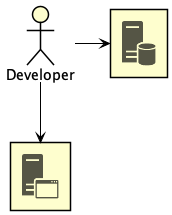
\includegraphics[width=0.25\textwidth]{diagrams/iron-age}
}
\only<2>{
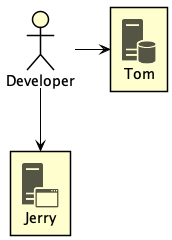
\includegraphics[width=0.25\textwidth]{diagrams/iron-age-names}
}
\end{center}
}

\point[Introducing...]{The \highlight{Cloud Age}}

\point[The Cloud Age]{
\begin{center}
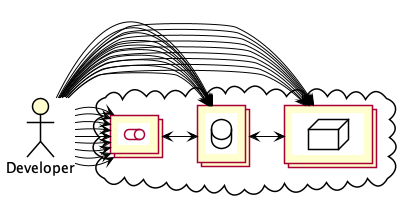
\includegraphics[width=0.5\textwidth]{diagrams/cloud-age}
\end{center}
}

\point[When faced with complexity]{Automate it!}

\begin{frame}{The larger story}

\begin{description}[<+->][leftmargin=!,labelwidth=\widthof{Data}]
    \item[Server Config] Config Management
    \item[Application Config] Config Files
    \item[Provisioning] Infrastructure Code
    \item[Building] Continuous Integration
    \item[Deployment] Continuous Deployment
    \item[Testing] Automated Tests
    \item[Database Administration] Schema Migration
    \item[Specifications] Behaviour Driven Development
\end{description}

\end{frame}

\begin{frame}
\large
\only<1->{
\begin{defn}[Infrastructure Code]
    Code that provisions \highlight{infrastructure resources}.
\end{defn}}

\only<2->{
\begin{defn}[Infrastructure Resources]
    Compute resources, networking resources, and storage resources.
\end{defn}}
\end{frame}

\point[Infrastructure Code]%
{   
\begin{center}\Large
    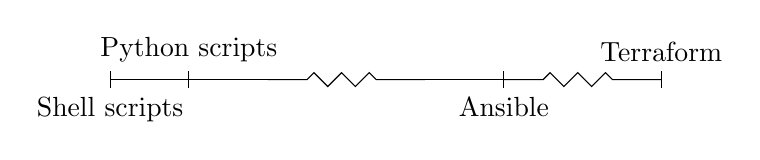
\begin{tikzpicture}[
        snake=zigzag,line before snake=5mm,line after snake=5mm
      ]
      \draw (0,0) -- (2,0);
      \draw[snake] (2,0) -- (4,0);
      \draw (4,0) -- (5,0);
      \draw[snake] (5,0) -- (7,0);
  
      \foreach \x in {0,1,5,7} \draw (\x cm,3pt) -- (\x cm,-3pt);
  
       \draw (0,0) node[below=3pt] {Shell scripts} node[above=3pt] {};
       \draw (1,0) node[below=3pt] {} node[above=3pt] {Python scripts};
       \draw (3,0) node[below=3pt] {} node[above=3pt] {};
       \draw (4,0) node[below=3pt] {} node[above=3pt] {};
       \draw (5,0) node[below=3pt] {Ansible} node[above=3pt] {};
       \draw (6,0) node[below=3pt] {} node[above=3pt] {};
       \draw (7,0) node[below=3pt] {} node[above=3pt] {Terraform};
    \end{tikzpicture}
\end{center}
}

\begin{frame}[fragile]
\begin{code}[language=bash]{}
#!/bin/bash

SG=$(aws ec2 create-security-group ...)

aws ec2 authorize-security-group-ingress --group-id "$SG"

INST=$(aws ec2 run-instances --security-group-ids "$SG" \
         --instance-type t2.micro)
\end{code}
\end{frame}

\begin{frame}[fragile]
\begin{code}[language=python]{}
import boto3

def create_instance():
    ec2_client = boto3.client("ec2", region_name="us-east-1")
    response = ec2.create_security_group(...)
    security_group_id = response['GroupId']

    data = ec2.authorize_security_group_ingress(...)

    instance = ec2_client.run_instances(
        SecurityGroups=[security_group_id],
        InstanceType="t2.micro",
        ...
    )
\end{code}
\end{frame}

\begin{frame}[fragile]
\begin{code}[language=terraform]{}
resource "aws_instance" "hextris-server" {
    instance_type = "t2.micro"
    security_groups = [aws_security_group.hextris-server.name]
    ...
}

resource "aws_security_group" "hextris-server" {
    ingress {
        from_port = 80
        to_port = 80
        ...
    }
    ...
}
\end{code}
\end{frame}

\question{Notice anything different?}

\point[The \textsl{main} difference]{Imperative vs. Declaritive}

\point[Infrastructure Code]{
\Large
\begin{itemize}[<+->]
    \item Provisions and manages \highlight{infrastructure resources}.
    \item Only one part of the movement to \highlight{automate} the complexities of development.
    \item Ranges from simple shell scripts up to\dots?
    \item Tendancy to be \highlight{declaritive}.
\end{itemize}
}

\point[Typo?]{Infrastructure Code $\neq$ Infrastructure \highlight{as} Code}

\definition{Infrastructure as Code}%
{Following the same \highlight{good coding practices} to manage Infrastructure Code as standard code.}

\point[Warning!]{Infrastructure as Code still \highlight{early} and quite \highlight{bad}.}

\question{What are \highlight{coding practices}?}

\point[Good Coding Practice \#1]{\highlight{Everything} as code}

\begin{frame}[fragile]
\begin{code}[language=shell]{}
#!/bin/bash

./download-dependencies
./build-resources
cp -r output/* artifacts/
\end{code}

\only<2>{\bash{cp: directory artifacts does not exist}}
\end{frame}

\begin{frame}[fragile]
\begin{code}[language=terraform]{}
resource "aws_instance" "hextris-server" {
    instance_type = "t2.micro"
    security_groups = ["sg-6400"]
    ...
}
\end{code}
\end{frame}

\begin{frame}[fragile]
\begin{code}[language=terraform]{}
resource "aws_instance" "hextris-server" {
    instance_type = "t2.micro"
    security_groups = [aws_security_group.hextris-server.name]
    ...
}

resource "aws_security_group" "hextris-server" {
    ingress {
        from_port = 80
        to_port = 80
        ...
    }
    ...
}
\end{code}
\end{frame}

\point[Good Coding Practice \#2]{Version control}

\point[Benefits]{
\begin{enumerate}
    \item Reproducable.
    \item Restorable.
    \item Accountable.
\end{enumerate}
}

\point[Good Coding Practice \#3]{Automation}

\point[Good Coding Practice \#4]{Re-use Code}

\point[Good Coding Practice \#5]{Testing}



\end{document}